\documentclass{article}
\usepackage[utf8]{inputenc}
\usepackage{amsmath, amsthm, amssymb, mathpazo, isomath, mathtools}
\usepackage{subcaption,graphicx,pgfplots}
\usepackage{xcolor}

\begin{document}

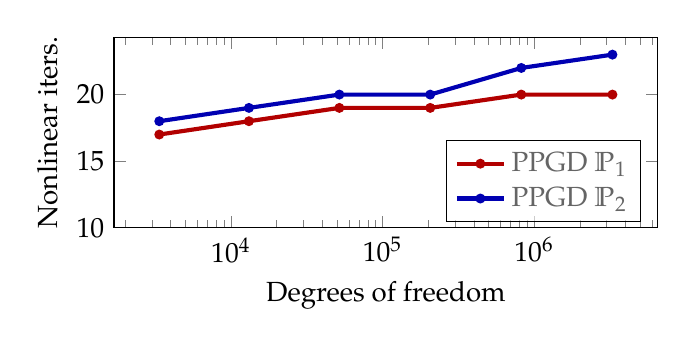
\begin{tikzpicture}
        \begin{semilogxaxis}[xlabel=Degrees of freedom, ylabel=Nonlinear iters., width=0.7\textwidth, height=4cm, ymin=10, legend style={fill opacity=0.6, legend cell align=left, legend pos=south east}, legend columns=1]
            \addplot[red!70!black, style={ mark options={draw opacity=1.0, fill opacity=1.0, mark size=1pt}}, mark=*, line width=1.5] coordinates
            {(3362, 17)(13122, 18)(51842, 19)(206082, 19)(821762, 20)(3281922, 20)};
            \addplot[blue!70!black, style={ mark options={draw opacity=1.0, fill opacity=1.0, mark size=1pt}}, mark=*, line width=1.5] coordinates
            {(3362, 18)(13122, 19)(51842, 20)(206082, 20)(821762, 22)(3281922, 23)};
            \legend{PPGD $\mathbb P_1$, PPGD $\mathbb P_2$}
        \end{semilogxaxis}
    \end{tikzpicture}

\end{document}